\documentclass[border=10pt]{standalone}
\usepackage{circuitikz}
\usepackage{tikz}
\usetikzlibrary{calc, positioning, arrows.meta, shapes.geometric, shadows}

\begin{document}
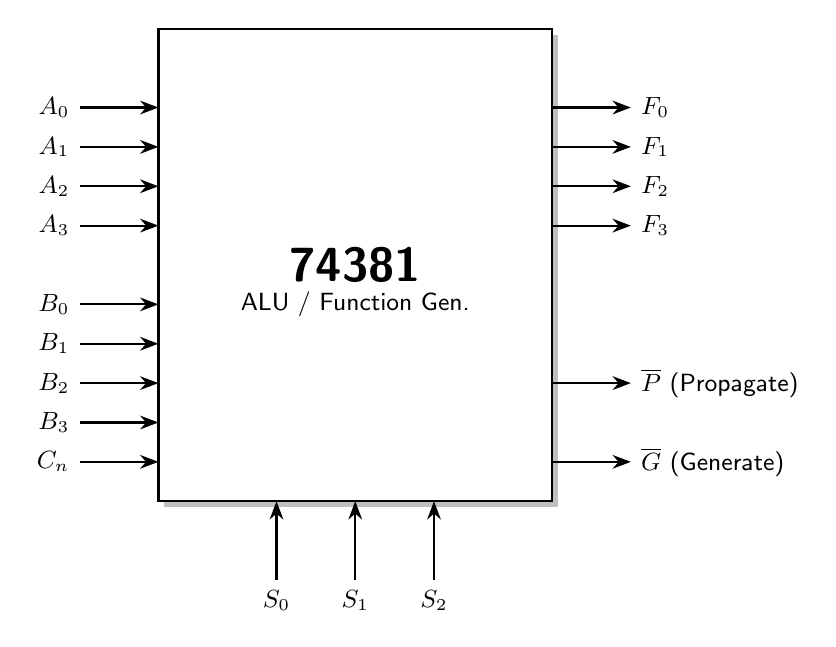
\begin{tikzpicture}[
    >=Stealth, 
    thick, 
    font=\sffamily\small
]

    % Main Block Body
    \draw[fill=white, drop shadow] 
        (0, 0) rectangle (5, 6);
    
    % Label
    \node at (2.5, 3) {\LARGE \textbf{74381}};
    \node at (2.5, 2.5) {ALU / Function Gen.};

    % Inputs (Left Side - A and B)
    % A Inputs (Top Left)
    \draw[<-] (0, 5) -- (-1, 5) node[left] {$A_0$};
    \draw[<-] (0, 4.5) -- (-1, 4.5) node[left] {$A_1$};
    \draw[<-] (0, 4) -- (-1, 4) node[left] {$A_2$};
    \draw[<-] (0, 3.5) -- (-1, 3.5) node[left] {$A_3$};

    % B Inputs (Bottom Left)
    \draw[<-] (0, 2.5) -- (-1, 2.5) node[left] {$B_0$};
    \draw[<-] (0, 2) -- (-1, 2) node[left] {$B_1$};
    \draw[<-] (0, 1.5) -- (-1, 1.5) node[left] {$B_2$};
    \draw[<-] (0, 1) -- (-1, 1) node[left] {$B_3$};

    % Select Inputs (Bottom)
    \draw[<-] (1.5, 0) -- (1.5, -1) node[below] {$S_0$};
    \draw[<-] (2.5, 0) -- (2.5, -1) node[below] {$S_1$};
    \draw[<-] (3.5, 0) -- (3.5, -1) node[below] {$S_2$};

    % Carry In (Left - Separate or bottom?) Standard usually bottom left or side.
    % Let's put Carry In on the left separate spot or bottom.
    % 74381 has Cn.
    \draw[<-] (0, 0.5) -- (-1, 0.5) node[left] {$C_n$};


    % Outputs (Right Side)
    % F Outputs
    \draw[->] (5, 5) -- (6, 5) node[right] {$F_0$};
    \draw[->] (5, 4.5) -- (6, 4.5) node[right] {$F_1$};
    \draw[->] (5, 4) -- (6, 4) node[right] {$F_2$};
    \draw[->] (5, 3.5) -- (6, 3.5) node[right] {$F_3$};

    % Propagate and Generate (Right Side - Bottom)
    % Convention: Active Low P and G often. We'll label as \bar{P} and \bar{G} or just P/G depending on user pref.
    % Standard 74381 is active low P, G.
    \draw[->] (5, 1.5) -- (6, 1.5) node[right] {$\overline{P}$ (Propagate)};
    \draw[->] (5, 0.5) -- (6, 0.5) node[right] {$\overline{G}$ (Generate)};

\end{tikzpicture}
\end{document}
